\documentclass[aapm,ajp,amsmath,amssymb,reprint]{revtex4-2}

\usepackage{graphicx}
\usepackage{hyperref}
\hypersetup{colorlinks=true,urlcolor=blue,linkcolor=black,citecolor=black}

\begin{document}

\title{The Levitron Lab: An Interactive Curriculum for Magnetic Levitation Physics}

\author{Saleem Aldajani}
\email{saldajani@mit.edu}
\affiliation{Massachusetts Institute of Technology, Cambridge, Massachusetts 02139, USA}

\date{\today}

\begin{abstract}
We describe \emph{The Levitron Lab}, a browser-based collection of interactive simulations that teach how different magnetic levitation toys work by climbing a dimensionality ladder from Earnshaw's theorem to full rigid-body and driven-rotor dynamics. Each of five modules foregrounds a live, animated levitating object with sliders on every physical parameter, diagnostic plots, and inline equations. Feedback modules implement full PID control with live Jacobian eigenvalues; the gyroscopic module implements the symmetric-top nutation analysis from the author's MIT 8.223 project. The tool is open source, runs offline, and deploys in one click via GitHub Codespaces (\url{https://github.com/saldajani/levitron-lab}). Supplementary interactive materials are available at the repository and in the accompanying video.
\end{abstract}

\maketitle

\section{Introduction}
\label{sec:intro}

Earnshaw's theorem forbids stable equilibrium for a magnetic dipole in a static field: wherever forces balance, the potential is a saddle~\cite{simon}. Yet levitating globes, spinning tops, and motor-driven floaters are sold as toys. Each evades the theorem by a distinct mechanism: time-varying feedback fields; gyroscopic spin; or frequency-locked rotation in a driven field~\cite{berry,hermansen,doff}.

The Levitron Lab presents all three escape routes in one curriculum, ordered by \emph{which directions are unstable}---a classification articulated in conversation with an experimental atomic physicist who keeps a classic Levitron on his desk as a tabletop model of a magnetic atom trap~\cite{ketterle}.

\section{Earnshaw's theorem and the three escape routes}
\label{sec:earnshaw}

Module~0 places a free magnet above a fixed magnet. The user hunts for $F(z)=0$ and discovers $\partial^2 U/\partial z^2<0$: passive levitation is impossible (Fig.~\ref{fig:earnshaw}).

\begin{figure}[htbp]
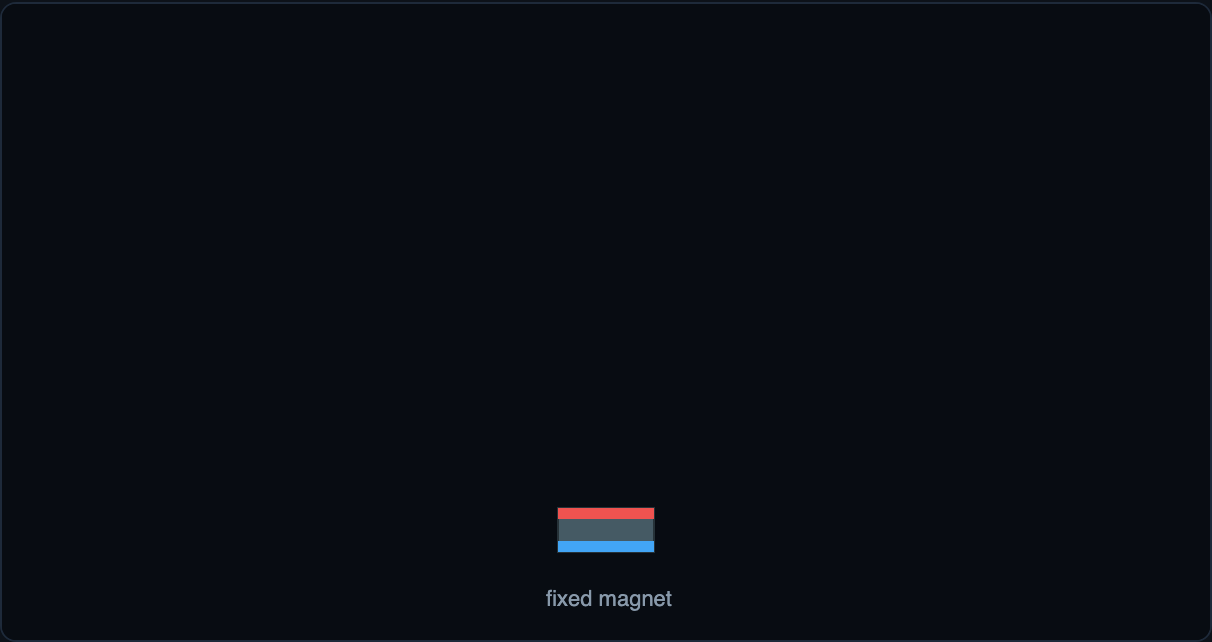
\includegraphics[width=\linewidth]{figures/fig_earnshaw_saddle.png}
\caption{\label{fig:earnshaw}Earnshaw primer: the free magnet cannot rest at the force balance --- an unstable hilltop, not a bowl.}
\end{figure}

The three escape routes previewed are: (1)~active feedback (Modules~1--2); (2)~gyroscopic spin (Module~3); (3)~driven rotation (Module~4).

\section{The five modules and implementation}
\label{sec:modules}

The application is built in React, TypeScript, and \texttt{three.js}. Physics integrates on a fixed $1$\,ms timestep decoupled from rendering; feedback modules use semi-implicit Euler; rigid-body modules use RK4.

\subsection{One- and two-dimensional feedback}

Module~1 models the floating-globe class: stable horizontally, unstable in $z$, corrected by PID control
\begin{equation}
I=\mathrm{clamp}\!\left(K_p e + K_i\!\int e\,dt + K_d \dot e,\,0,\,I_{\max}\right).
\end{equation}
Module~2 is the mathematically distinct sibling: stable in $z$, unstable in $x$ and $y$, corrected by four horizontal coils. Both modules compute the closed-loop Jacobian and display eigenvalues live (Fig.~\ref{fig:eigs}).

\begin{figure}[htbp]
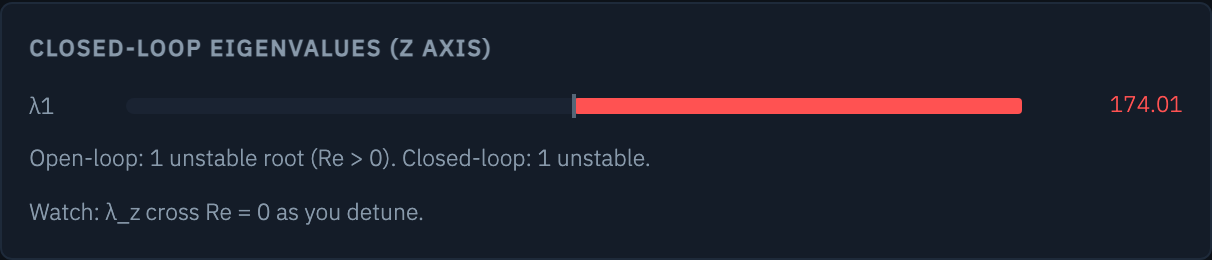
\includegraphics[width=0.48\linewidth]{figures/fig_feedback1d_eigs.png}
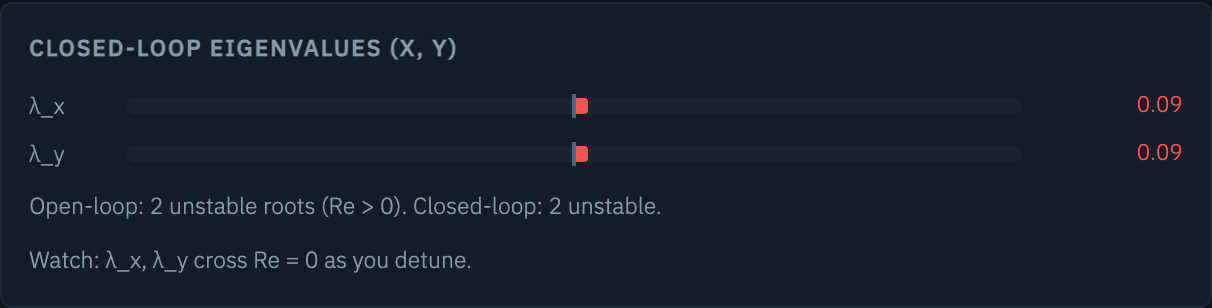
\includegraphics[width=0.48\linewidth]{figures/fig_feedback2d_eigs.png}
\caption{\label{fig:eigs}Closed-loop eigenvalues for Module~1 ($z$ instability tamed) and Module~2 ($x,y$ instabilities tamed). Open-loop unstable roots cross $\mathrm{Re}\,\lambda=0$ when detuned.}
\end{figure}

Thermal drift with $K_i=0$ produces visible steady-state sag below setpoint; raising $K_i$ eliminates the offset --- a teaching point tied to real levitating-globe trim pots.

\subsection{Dynamical rotor levitation}

Module~4 integrates a floater in a motor-driven rotor field~\cite{hermansen,doff,apsfocus}. Trapping onset is governed by rotor geometry; the module displays $U_f(z_f)$ morphing as the lateral-displacement parameter crosses its critical value (Fig.~\ref{fig:rotor}).

\begin{figure}[htbp]
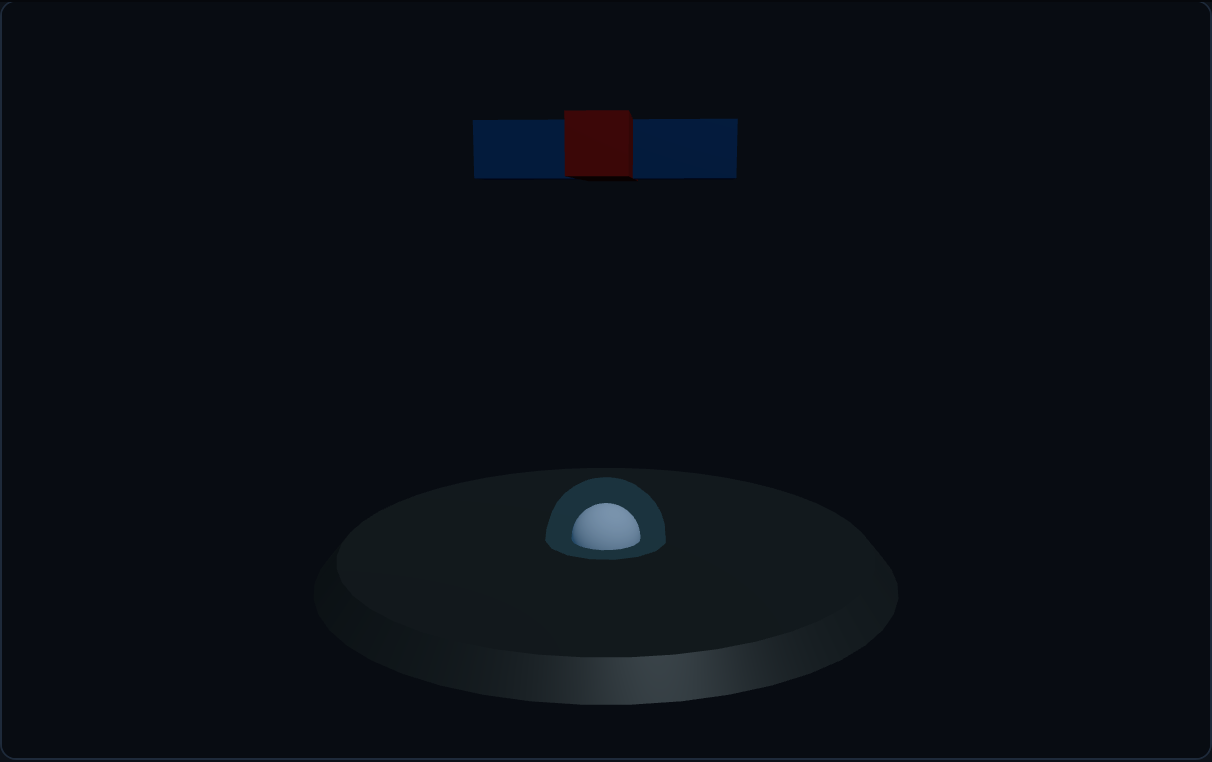
\includegraphics[width=0.48\linewidth]{figures/fig_rotor_trap.png}
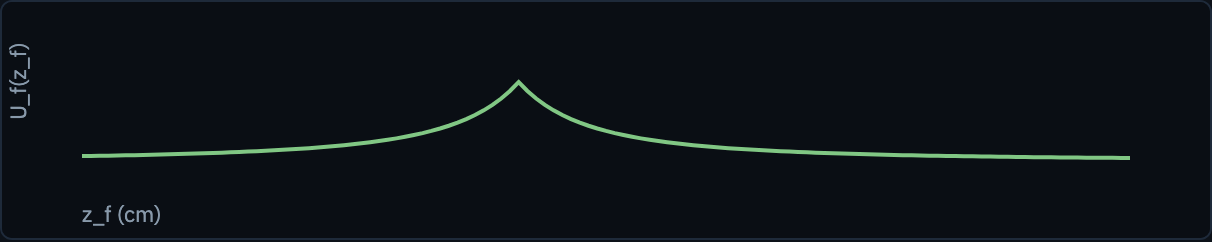
\includegraphics[width=0.48\linewidth]{figures/fig_rotor_potential.png}
\caption{\label{fig:rotor}Dynamical rotor module: frequency-locked floater (left) and floater potential $U_f(z_f)$ (right).}
\end{figure}

\section{The gyroscopic top and the 8.223 symmetric-top analysis}
\label{sec:gyro}

The classic Levitron is stabilized by angular momentum and magnetic force alone~\cite{simon,berry}. Module~3 implements the symmetric-top mechanics developed in the author's MIT 8.223 project~\cite{aldajani823,video}.

\subsection{Lagrangian, conserved momenta, and precession roots}

For a symmetric top with Euler angles $(\varphi,\theta,\psi)$ (precession, nutation, spin), the conserved momenta are
\begin{align}
p_\psi &= I_s(\dot\psi+\dot\varphi\cos\theta), \\
p_\varphi &= (I_p\sin^2\theta+I_s\cos^2\theta)\dot\varphi + I_s\dot\psi\cos\theta.
\end{align}
At fixed $\theta$, there are slow and fast precession roots; the slow root satisfies $\dot\varphi_{\mathrm{slow}}=mgl/p_\psi$. Launching at the slow-precession equilibrium with $\dot\theta=0$ and $\cos\theta_{\mathrm{stable}}=p_\varphi/p_\psi$ is essential --- arbitrary transverse angular velocity at $\theta=0$ ejects the top immediately.

\subsection{Restoring potential and bounded nutation}

Nutation satisfies an effective one-dimensional equation with potential
\begin{equation}
U_{\mathrm{res}}(\theta)=\frac{p_\psi^2}{2I_s}+\frac{(p_\varphi-p_\psi\cos\theta)^2}{2I_p\sin^2\theta}+V_{\mathrm{eff}}(\theta),
\end{equation}
where $V_{\mathrm{eff}}$ combines gravity and magnetic upright bias (replacing $mgl\cos\theta$ in the gravitational-top form). Bounded nutation requires $\theta_{\min}<\theta<\theta_{\max}$ at the turning points of $U_{\mathrm{res}}$ (Fig.~\ref{fig:ures}). The device ``works only when nice and upright'': the allowable cone half-angle $\theta_c$ shrinks as spin drops toward $\omega_{\min}$ or as the field weakens with temperature.

\begin{figure*}[htbp]
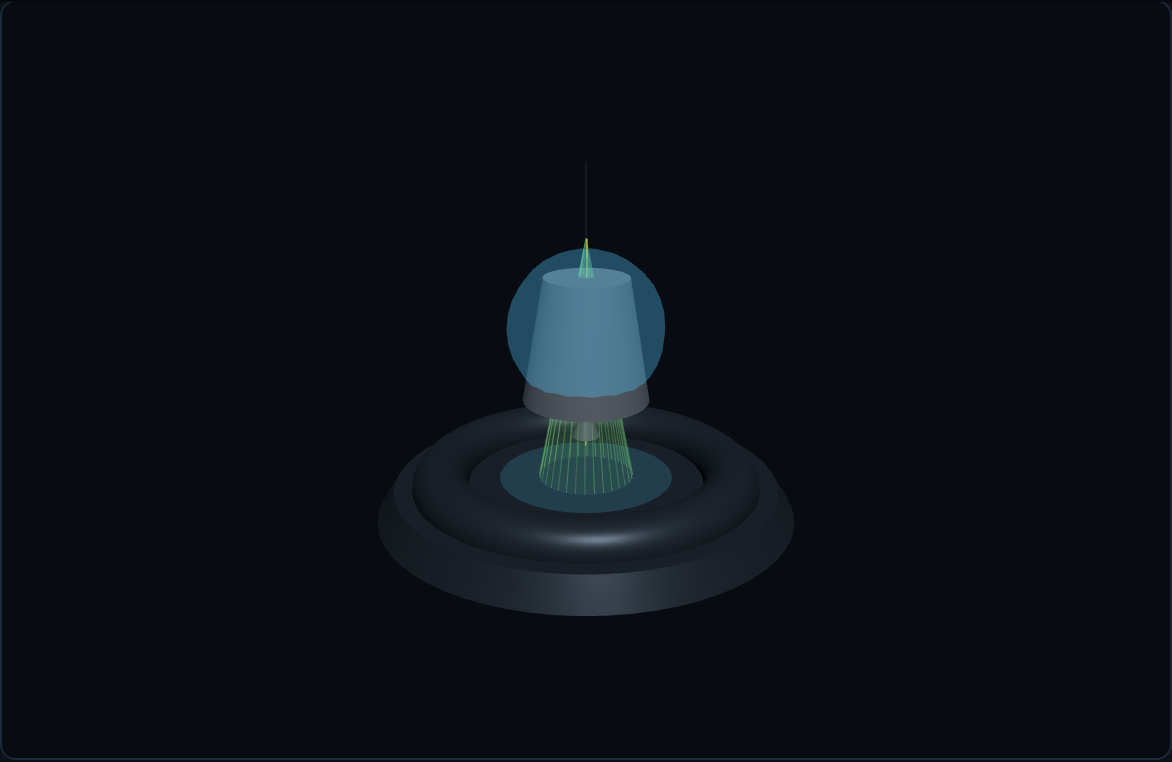
\includegraphics[width=0.55\linewidth]{figures/fig_gyro_stable.png}
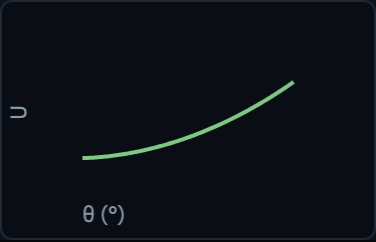
\includegraphics[width=0.42\linewidth]{figures/fig_gyro_potential.png}
\caption{\label{fig:gyro}(Left) Stable gyroscopic Levitron with nutation cone and symmetry axis. (Right) $U_{\mathrm{res}}(\theta)$ showing the restoring well; $\theta_{\min}<\theta<\theta_{\max}$.}
\end{figure*}

\begin{figure}[htbp]
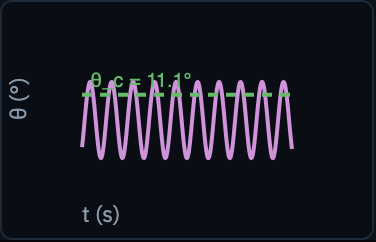
\includegraphics[width=\linewidth]{figures/fig_gyro_theta_trace.png}
\caption{\label{fig:theta}Nutation angle $\theta(t)$: bounded nodding when stable; diverging growth before crash.}
\end{figure}

The spin-rate window ($\omega_{\min}\!\approx\!19$~rps for ferrite) and nutation cone are \emph{both} required: the window ensures adiabatic following of the field (Berry phase~\cite{berry}); the cone keeps the axis upright enough for that following to hold. Startup diagnostics verify $p_\psi^2\gg 4mglI_p\cos\theta$ and that $U_{\mathrm{res}}$ possesses a local minimum before integration begins.

\section{From toy to atom trap}
\label{sec:atom}

A neutral atom with spin angular momentum is a microscopic gyroscope; magnetic trapping uses the same adiabatic-invariant logic as the Levitron~\cite{ketterle,berry}. The tool includes a dedicated page drawing this correspondence explicitly.

\section{Classroom use and availability}
\label{sec:avail}

The Levitron Lab runs fully client-side with no backend. GitHub Codespaces provides one-click deployment: \texttt{npm install} and \texttt{npm run dev -- --host} start automatically. Figure capture for papers uses \texttt{npm run figures} (Playwright). See \url{https://github.com/saldajani/levitron-lab}.

\section{Conclusion}
\label{sec:conclusion}

By rendering the levitating body alongside the equations that govern it, and by ordering devices according to unstable dimensionality, The Levitron Lab turns familiar toys into a unified quantitative curriculum from Earnshaw's prohibition to atom-trap analogies.

\begin{acknowledgments}
The author thanks W.~Ketterle for the conversation that motivated this work.
\end{acknowledgments}

\begin{thebibliography}{99}
\bibitem{aldajani823} S.~Aldajani and Alowayed, ``Understanding the Levitron Through the Analysis of a Symmetric Spinning Top in a Gravitational Field,'' MIT 8.223 Classical Mechanics III project report (author's prior work). \url{http://goo.gl/c5u3lk}
\bibitem{video} S.~Aldajani, demonstration video of the symmetric-top Levitron analysis. \url{https://www.youtube.com/watch?v=1LHwq_g06fE}
\bibitem{simon} M.~D.~Simon, L.~O.~Heflinger, and S.~L.~Ridgway, Am.\ J.\ Phys.\ \textbf{65}, 286 (1997). \url{https://www.physics.ucla.edu/marty/levitron/spinstab.pdf}
\bibitem{berry} M.~V.~Berry, Proc.\ R.\ Soc.\ Lond.\ A \textbf{452}, 1207 (1996).
\bibitem{hermansen} J.~M.~Hermansen \textit{et al.}, Phys.\ Rev.\ Applied \textbf{20}, 044036 (2023).
\bibitem{doff} A.~Doff and R.~M.~Szmoski, arXiv:2506.23268. \url{https://arxiv.org/html/2506.23268v2}
\bibitem{apsfocus} R.~Berkowitz, Physics (APS) \textbf{16}, 177 (2023).
\bibitem{mitviz} MIT VIZ Group. \url{https://web.mit.edu/viz/levitron/Physics.html}
\bibitem{wiki} ``Spin-stabilized magnetic levitation,'' Wikipedia.
\bibitem{ketterle} W.~Ketterle, personal communication, MIT, June 2026.
\end{thebibliography}

\end{document}
